\section{Метод главных компонент}


Основной задачей метода главных компонент (он же PCA от Principal Component Analysis)  является минимизация ошибки восстановления данных, если они проецируются на подпространство меньшей размерности $k<d$, где $d$ - исходная размерность, а $k$ - уменьшенная. Функция потерь в этом случае задаётся как:

\[
L = \| \mathbf{X} - \mathbf{X}_{\text{proj}} \|_F^2,
\]

где:

\begin{itemize}
    \item \( \mathbf{X} \in \mathbb{R}^{n \times d} \) — исходная центрированная матрица данных, состоящая из $n$ векторов-строк из пространства размерности $d$;
    \item \( \mathbf{X}_{\text{proj}} = \mathbf{X} \mathbf{W} \mathbf{W}^\top \) — проекция данных на подпространство, заданное матрицей \( \mathbf{W} \);
    \item \( \| \cdot \|_F^2 \) — фробениусова норма, измеряющая суммарное отклонение всех точек данных от их проекций.
\end{itemize}

PCA минимизирует \( L \) путём выбора такого \( k \)-мерного подпространства, которое сохраняет максимальную часть дисперсии данных. \\

\textbf{Задача 1}. Докажите, что алгоритм последовательного построения главных компонент обладает свойством жадного отбора: локальные минимизации функции потерь путем добавления следующих главных компонент ведут к глобальной минимизации функции потерь для заданного числа главных компонент. 

\textit{Решение}
Действительно, алгоритм PCA заключается в следующем:\\

0. Если число главных компонент равно нулю, так, что мы проецируем данные на нульмерное пространство-точку, то оптимальной точкой будет начало координат, минимизирующее фробениусову норму

1. Выбираем первую главную компоненту (первый вектор базиса) так, чтобы выборочная дисперсия вдоль данной компоненты была минимальна. 

2. Вторую главную компоненту выбираем так, чтобы дисперсия данных вдоль нее была максимальна при условии ортогональности первой главной компоненте.

3. Аналогично выбираем третью главную компонету при условии ортогональности первой и второй. Далее действуем аналогично.


На каждом шаге будет получаться локально оптимальный выбор базиса главных компонент, при проекцировании данных на который функция потерь будет минимальна. Но поскольку каждый такой локальный базис является подбазисом объемлющего базиса и бОльшего числа главных компонент, который является глобально оптимальным, мы получаем, что локальные оптимизации функции потерь путем последовательного построения главных компонент приводят к глобально оптимальному базису.\\

\textbf{Задача 2}. Покажите, что $k$-ая главная компонента "важнее"  $k+1$ главной компоненты с точки зрения минимизации функции потерь.\\

\textit{Решение}. Это следует из вида функции потерь для $k$ главных компонент:

\[
\sum_{i=k+1}^d \lambda_i,
\]
где $\lambda_i$ - собственные числа ковариационной матрицы $\mathbf{\Sigma} = \frac{1}{n} \mathbf{X}^\top \mathbf{X}$, а также свойства собственных чисел: $ \lambda_{i+1} \leq \lambda_i$

\section{Автокодировщики в сравнении с PCA}

Автокодировщики представляют собой нейронные сети, предназначенные для обучения компактных представлений данных. Суть автокодировщика заключается в том, что он обучается на реконструкции исходных данных с помощью более компактной внутренней репрезентации (латентное пространство). В отличие от PCA, автокодировщики могут обучаться не только на линейных, но и на нелинейных зависимостях между признаками, что делает их более гибкими и мощными инструментами для снижения размерности.

Автокодировщик состоит из двух частей: энкодера и декодера. Энкодер преобразует исходные данные в скрытое представление (латентное пространство), а декодер восстанавливает исходные данные из этого представления. Обучение автокодировщика заключается в минимизации ошибки восстановления между исходными данными и их реконструкцией.

На лицо видна аналогия между PCA и автокодировщиками: 

1. Оба метода сжимают исходные данные: PCA в матрицу признаков меньшей размерности, а автокодировщик - в латентное пространство

2. Оба метода минимизируют фробениусову норму входной и выходной матриц: у PCA это матрица признаков, а у автокодировщиков, как правило, эта матрица (или тензор) представляет из себя изображение.

Однако у PCA есть полезные свойства, которыми не обладает обыкновенный автокодировщик: 

1. Главные компоненты отсортированы по обыванию их "важности" по минимизации функции потерь. Это позволяет жадным образом отбирать самые необходимые главные компоненты для сжатия данных.

2. Главные компоненты ортогональны и статистически независимы. Это повышает интерпретабельность PCA.



\section{Алгоритм PCAАE}

Оказывается можно построить автокодировщик, который обладает приведенными выше свойствами. Следуя авторам, будем называть его PCAAE (Principal Component Analysis Autoencoder) или PCA-автокодировщик.

Перед тем как описать PCA-автокодировщик, сначала определим некоторые обозначения. Пусть \( \mathbf{X} \) — это пространство данных, в общем случае мы будем рассматривать изображения размера \( n \times n \), то есть \( \mathbf{X} = \mathbb{R}^{n \times n} \). Обозначим латентное пространство как \( \mathbf{Z} = \mathbb{R}^d \), где \( d \) — размерность этого латентного пространства. Обозначим кодировщик как \( E: \mathbf{X} \to \mathbf{Z} \), а декодировщик как \( D: \mathbf{X} \to \mathbf{Z} \). Обозначим \( z_i \) как \( i \)-й компонент вектора \( \mathbf{z} \). Пусть \( y = D \circ E(\mathbf{x}) \) — это вывод автокодировщика. Кроме того, обозначим \( \mathbf{x}^{(i)} \) как \( i \)-й образец данных, а его код \( \mathbf{z}^{(i)} = E(\mathbf{x}^{(i)}) \). Наконец, будем обозначать \( i \)-ю версию кодировщика как \( E^{(i)}: \mathbf{X} \to \mathbb{R}^i \), и аналогично для декодировщика.

Теперь опишем основную идею и алгоритм PCA-автокодировщика. Как мы уже объяснили, есть два центральных вопроса, которые мы должны решить для определения PCA-автокодировщика:
\begin{itemize}
    \item Что мы понимаем под «увеличением важности» компонент латентного пространства, и как мы можем это наложить?
    \item Как мы можем обеспечить независимость латентных кодов?
\end{itemize}

В случае PCA важность определяется вариативностью данных вдоль оси, однако такое определение трудно применить к автокодировщику, так как в процессе обучения, как правило, все размерности латентного пространства заполняются. Таким образом, просто выполнить PCA на латентном пространстве не получится.

Поэтому мы вводим понятие важности, обучая серию автокодировщиков с увеличивающимся размером латентного пространства, начиная с латентного пространства размерности 1 (скаляр). В этом первом автокодировщике мы можем предположить, что информация наибольшей «важности» будет закодирована, в смысле минимизации потерь \( \ell_2 \). Например, это может быть средний цвет фона. Затем мы увеличиваем размер латентного пространства на 1, сохраняя ту же первую компоненту из предыдущего обучения: обучается только вторая компонента. Этот процесс повторяется итеративно, пока не будет достигнут предустановленный размер \( d_{\max} \). Заметим, что на каждой итерации предыдущий декодировщик отбрасывается, и новый обучается с нуля. Действительно, мы хотим наложить структуру на латентное пространство через обучение кодировщика, но декодировщик должен иметь возможность делать это по своему усмотрению.

Мы решаем второй вопрос, как наложить независимость на латентные коды, следующим образом. Для этого потребуем, чтобы величина ковариации каждой компоненты латентного пространства была как можно меньше. Мы можем достичь этого, добавив дополнительный член в функцию потерь автокодировщика, который будет учитывать эту зависимость. Предположим, что мы добавляем компоненту \( k \) в латентное пространство. Тогда для пакета данных размером \( M \), \( X = \{ \mathbf{x}^{(1)}, \dots, \mathbf{x}^{(M)} \} \), мы можем вычислить ковариацию по формуле:
\[
L_{\text{cov}}(X) = \sum_{i=1}^{k-1} \left[ \frac{1}{M} \sum_{j=1}^{M} \left( z_i^{(j)} z_k^{(j)} - \frac{1}{M} \sum_{j=1}^{M} z_i^{(j)} \sum_{j=1}^{M} z_k^{(j)} \right) \right].
\]

Чтобы упросить задачу, мы до латентного слоя применим batch normalisation, тогда получим: 

$$L_{\text{cov}}(X) = \frac{1}{M} \sum_{i=1}^{k-1} \sum_{j=1}^{M} z_i^{(j)} z_k^{(j)}
$$\\

\textbf{Задача 3}. Докажите утверждение выше.\\

\textit{Решение}.
Формула для batch normalisation имеет вид:
\[
y_i = \gamma \left( \frac{x_i - \mu}{\sqrt{\sigma^2 + \epsilon}} \right)
\]
Таким образом получается центрированный набор данных с нулевым средним, поэтому  $\sum_{j=1}^{M} z_i^{(j)} = 0$.\\

Итоговая функция потерь будет иметь вид:

$$L(X) = \frac{1}{M} \sum_{i=1}^{M} \left\| x^{(i)} - D \circ E(x^{(i)}) \right\|_2^2 + \lambda L_{\text{cov}}(X)
$$

Минимизируя эту функцию, мы, во-первых, добиваемся того, чтобы выходное изображение было похоже на входное, во-вторых, добиваемся как можно меньшей статистической зависимости между компонентами латентного пространства. 

\begin{thebibliography}{99}


\bibitem{article1} Saïd Ladjal, Alasdair Newson \textit{A PCA-Like Autoencoder}, arviv.org  2 Apr 2019.

\bibitem{article2} Saïd Ladjal, Alasdair Newson \textit{PCAAE: Principal Component Analysis Autoencoder for organising the latent space of generative networks}, arviv.org 14 Jun 2020.

\end{thebibliography}

\section{Введение в метод главных компонент(PCA)}
\textbf{Метод главных компонент (Principal Component Analysis, PCA)} — это статистический метод, используемый для снижения размерности данных с сохранением наиболее значимой информации. PCA находит новые признаки (главные компоненты), 
которые представляют собой линейные комбинации исходных признаков, причем эти компоненты ортогональны и ранжированы по величине объясняемой дисперсии.
\textbf{Основные этапы метода:} \\
1. \textbf{Центрирование данных}:\\ Данные центрируются так, чтобы среднее значение каждой переменной было равно нулю:
$$
X_c=X-\bar{X},
$$
где $X$ - исходная матрица данных (размер $n \times p$ ), $\bar{X}$ - вектор средних значений по столбцам.\\
2. \textbf{Построение ковариационной матрицы}: \\ Вычисляется ковариационная матрица:
$$
\Sigma=\frac{1}{n-1} X_c^T X_c
$$
где $\Sigma$ - симметричная матрица размером $p \times p$.\\
3. \textbf{Собственные значения и собственные векторы}: \\ Решается задача нахождения собственных значений и собственных векторов ковариационной матрицы:
$$
\Sigma \mathbf{v}_i=\lambda_i \mathbf{v}_i
$$
где $\lambda_i$ - собственные значения, $\mathbf{v}_i$ - соответствующие им собственные векторы.\\
4. \textbf{Ранжирование главных компонент}: \\ Собственные значения упорядочиваются по убыванию:
$$
\lambda_1 \geq \lambda_2 \geq \cdots \geq \lambda_p
$$
Первые несколько компонент, соответствующие самым большим собственным значениям, объясняют большую часть дисперсии данных.\\
5. \textbf{Проекция данных}: \\ Данные проецируются на главные компоненты:
$$
Z=X_c V_k,
$$
где $V_k$ — матрица $k$ собственных векторов, соответствующих $k$ наибольшим собственным значениям, $Z$ — матрица данных в пространстве главных компонент.

Свойства метода: \\
- Главные компоненты ортогональны:

$$
\mathbf{v}_i^T \mathbf{v}_j=0, \quad i \neq j
$$

- Дисперсия объясняется последовательностью собственных значений:

$$
\text { Объясненная дисперсия }=\frac{\sum_{i=1}^k \lambda_i}{\sum_{i=1}^p \lambda_i} \text {. }
$$

\section{Спектральный метод наименьших квадратов}

Ridge регрессия отделяет наименьшие собственные значения матрицы от нуля путем добаваления $\tau$ ко всем значениям. Аналогично PCA отделяет наименьшие собственные значения от 0, но другим методом, а именно просто не учитывает их(отбрасывает). Как будто в суммах вместо них просто стоят 0. Обобщение данного подхода и называется \textbf{Спектральным методом наименьших квадратов: } \\
Приведем алгоритм: 
\begin{enumerate}
    \item Строим SVD (Singular Value Decomposition) разложение, и упорядочиваем собственные значения по возрастанию: $\lambda_1 \geq \lambda_2 \geq \dots \geq \lambda_n$
    \item Есил среди них есть близкие к нулю значения(то есть у нас будет плохая обусловленность нашей матрицы $\Rightarrow$ мультиколлинеарность при обучении), то нам нужно найти способ отделения от 0 этих собственных значений: $\lambda_j \rightarrow \lambda^{'}_j \ \forall j = \overline{m,n}$. При этом собственные векторы не меняем. \\
    Рассмотим частные случаи:
    \begin{itemize}
        \item $\lambda^{'}_j = \lambda_j + \tau$ - гребневая регрессия (ridge regression)
        \item $\lambda^{'}_j = \lambda_j + I_{[j > m]}\infty$ - метод главных компонент (PCA)      
    \end{itemize}

    \item Применим формулы SVD для модификации МНК-решения: \\
     $$\alpha^{*} = \sum_{j =1}^{n} \frac{1}{\sqrt{\lambda_j}} u_j(v_j^Ty)  \rightarrow \alpha^{*} = \sum_{j =1}^{n} \frac{\sqrt{\lambda_j}}{\lambda^{'}_j} u_j(v_j^Ty)$$
     
     $$F\alpha^{*} = \sum_{j =1}^{n} v_j(v_j^Ty) \rightarrow F\alpha^{*} = \sum_{j =1}^{n} \frac{\lambda_j}{\lambda^{'}_j} v_j(v_j^Ty)
     $$
\end{enumerate}
Интуиция данного метода заключается в том, что мы вводим поправки для близких к нулю собсвенных значений ($\delta_j$) уменьшая вклад этих самых собственных значений. Эти паправки мы вольны варировать практически как угодно от небольших сдвигов (Ridge regression) и вплоть до $\infty$ (PCA).

\section{Задача низкорангового матричного разложения}
Сам метод PCA позволяет:
\begin{itemize}
    \item понижать размерность в задачах регресси/классификации
    \item генерировать новые признаки 
    \item формировать сжатое представление данных
\end{itemize}
Но это все задачи \textbf{низкорангового матричного представления}. \\
В общем случая задача следующая: \\
\textbf{Дано:} Матрица $Z = ||z_{ij}||_{n*m}, (i, j) \in \Omega \subset \{1, \dots, n\}*\{1, \dots, m\}$  \\ 
\textbf{Найти:} матрицы $X=||x_{it}||_{n*k}$ и $Y = ||y_{tj}||_{k*m}$ такие, что:  
$$
||Z-XY||^{2} = \sum_{(i,j) \in \Omega} (z_{ij} - \sum_t x_{it}*y_{tj})^2 \rightarrow \min_{X, Y}
$$
Из за дополнительных ограничений, мы вынуждены откзаться от SVD:
\begin{itemize}
    \item не квадратичная функция потерь
    \item неотрицательное матричное разложение $x_{it} \geq 0$, $y_{tj} \geq 0$
    \item разряженные данные: $|\Omega| \ll nm$
\end{itemize}

\section{Задачи на использование метода главных компонент}

\subsection{Задача 1: Вклад признаков в главные компоненты}
Пусть $X \in R_{n\times p}$ набор данных с n образцами (строками) и p признаками (столбцами). PCA стремится найти набор собственных векторов (главных компонент), которые максимизируют дисперсию данных при проецировании на эти векторы.

Задача состоит в том, чтобы математически оценить, какой вклад вносит каждый признак в главные компоненты, и проранжировать признаки в зависимости от их вклада.\\ \\
\textbf{Решение:}
Метод РСА ищет собственные векторы $\mathbf{v}_i$ и собственные значения $\lambda_i$ удовлетворяющие:

$$
\Sigma \mathbf{v}_i=\lambda_i \mathbf{v}_i,
$$


где $\lambda_i$ - величина дисперсии данных вдоль $\mathbf{v}_i$.
Собственные векторы $\mathbf{v}_i$ формируют матрицу $V=\left[\mathbf{v}_1, \mathbf{v}_2, \ldots, \mathbf{v}_p\right]$, где каждый столбец $\mathbf{v}_i$ указывает направления главных компонент.\\
\textbf{Вклад признака в главные компоненты:}\\

Каждый признак в $X$ вносит вклад в главные компоненты через веса собственных векторов $\mathbf{v}_i$ . Элементы $v_{i j}$ (где $v_{i j}-j$-й элемент $i$-го собственного вектора) определяют значимость $j$-го признака для $i$-й главной компоненты.

Вклад $j$-го признака в $i$-ю главную компоненту оценивается как квадрат соответствующего элемента $v_{i j}^2$ .\\

Общий вклад $j$-го признака во все главные компоненты можно найти, суммируя его взвешенные вклады с учётом дисперсий ( $\lambda_i$ ):\\
$j=\sum_{i=1}^p \lambda_i v_{i j}^2$.\\
Этот показатель учитывает как значимость признака для каждой компоненты $\left(v_{i j}^2\right)$, так и долю дисперсии, объясняемую компонентой ( $\lambda_i$ ).\\
На конкретном примере:
Пусть собственные вектора образуют матрицу V:

$$
V=\left[\begin{array}{cccc}
0.5 & 0.6 & 0.3 & 0.1 \\
0.4 & -0.7 & 0.2 & 0.5 \\
-0.6 & 0.2 & 0.7 & -0.4 \\
0.5 & 0.3 & -0.6 & -0.6
\end{array}\right]
$$
Собственные значения:

$$
\Lambda=\operatorname{diag}(4.0,2.5,1.2,0.3)
$$

Посчитаем вклад признака $1(j=1)$ :
Для этого берём первую строчку $V$ :

$$
v_{1, \cdot}=[0.5,0.6,0.3,0.1]
$$
Считаем:

$$
\begin{aligned}
\text { Contribution }_1 & =\left(0.5^2 \cdot 4.0\right)+\left(0.6^2 \cdot 2.5\right)+\left(0.3^2 \cdot 1.2\right)+\left(0.1^2 \cdot 0.3\right) \\
& =1.0+0.9+0.108+0.003=2.011
\end{aligned}
$$

То же самое повторяем для остальных строк и находим максимальное значение.
\subsection{Задача 2: Ошибка "реконструкции" PCA}
Пусть $X \in R_{n\times p}$ набор данных с $n$ образцами (строками) и $p$ признаками (столбцами), с помощью метода главных компонент нужно:
\begin{itemize}
\item{Спроецируйте данные в более низкоразмерное пространство, определяемое $k$ главными компонентами.}
\item {Реконструируйте исходные данные из пространства пониженной размерности.}
\item {Вычислите ошибку реконструкции и оцените, как она меняется в зависимости от количества сохраняемых компонент k.}
\end{itemize}
\textbf{Решение:}
Для реконструкции данных из $k$-мерного подпространства используется обратная проекция:

$$
\hat{X}=Z V_k^T+\bar{X}
$$


Здесь:
- $Z V_k^T$ возвращает проекцию данных в исходное $p$-мерное пространство.\\
- Добавление $\bar{X}$ восстанавливает исходное смещение данных. \\
Ошибка реконструкции должна показывать какую часть информации мы потеряли при использовании только $k$ компонент при репрезентации данных.\\
1. Определим ошибку реконструкции для одного объекта $x_i$ :

$$
E_i=\left\|x_i-\hat{x}_i\right\|^2=\left\|\left(x_i-\bar{X}\right)-\left(z_i V_k^{\top}\right)\right\|^2
$$

2. Обобщим на весь набор данных:

$$
E=\frac{1}{n \times p} \sum_{i=1}^n\left\|x_i-\hat{x}_i\right\|^2
$$

3. Заменим на выражение для $\hat{x}_i$:

$$
E=\frac{1}{n \times p} \sum_{i=1}^n\left\|x_i-\bar{X}-Z V_k^{\top}\right\|^2
$$
Мы получили выражение для ошибки реконструкции. Теперь докажем, что 
ошибка реконструкции $E$ уменьшается монотонно с $k$, и когда $k=p, E=0$.

1. Общая дисперсия данных - это след ковариационной матрицы, которая представляет собой сумму всех собственных значений:

$$
\text { Total Variance }=\sum_{j=1}^p \lambda_j
$$

2. Дисперсия, которую уловили $k$ компонент это:

$$
\text { Captured Variance }=\sum_{j=1}^k \lambda_j
$$

3. Ошибка реконструкции по сути является дисперсией, которую не удалось уловить, то есть просто:

$$
E=\text { Total Variance }- \text { Captured Variance }=\sum_{j=k+1}^p \lambda_j
$$

4. Так как $\lambda_1 \geq \lambda_2 \geq \cdots \geq \lambda_p \geq 0$, добавление большего числа компонент ( $k \rightarrow k+1$ ) уменьшает $E$ :

$$
\sum_{j=k+1}^p \lambda_j>\sum_{j=k+2}^p \lambda_j
$$

5. В тот момент, когда $k=p, \sum_{j=k+1}^p \lambda_j=0$ $\Rightarrow$ $E=0$.

\subsection{Задача 3: Построить критерий D-оптимальности для выбора лучших k-компонент }
Набор данных представляет собой матрицу $n \times p$, где n - число образцов (строк), а p - число признаков (столбцов). Введём критерий D-оптимальности, используемый для выбора подмножества точек из набора данных, которое максимизирует детерминант информационной матрицы.
$$
D_{opt} : max  det(X^{T}X)
$$

Ключевым свойством критерия D-оптимальности является то, что он максимизирует объём многомерной фигуры, которая получается из рассматриваемых признаков. \\
Нужно построить критерий D-оптимальности для выбора лучших 
k главных компонент, которые максимизируют детерминант объясненной дисперсии (или объём фигуры) в k-мерном подпространстве PCA. 

\textbf{Решение:}

Критерий D-оптимальности для подпространства $k$ задаётся максимизацией детерминанта информационной матрицы $\Lambda_k$ :

$$
D_{o p t}(k)=\max \operatorname{det}\left(\Lambda_k\right)
$$

Так как $\Lambda_k$ является диагональной матрицей, её детерминант равен произведению собственных значений:

$$
\operatorname{det}\left(\Lambda_k\right)=\prod_{i=1}^k \lambda_i
$$

Итак, наша задача сводится к выбору $k$-мерного подпространства (т.е. первых $k$ главных компонент), которые максимизируют произведение $\lambda_1 \cdot \lambda_2 \cdots \cdot \lambda_k$, что эквивалентно решению следующей задачи:

$$
\max _{V_k} \prod_{i=1}^k \lambda_i
$$


где $\lambda_i$ - собственные значения матрицы ковариации $\Sigma$.
Для вычисления $D_{\text {opt }}(k)$ :\\
\\
1. Центрируем данные:

$$
X_c=X-\bar{X},
$$


где $\bar{X}$ - матрица средних значений.\\
2. Вычисляем ковариационную матрицу:

$$
\Sigma=\frac{1}{n-1} X_c^T X_c
$$

3. Находим собственные значения $\lambda_1, \lambda_2, \ldots, \lambda_p$ и соответствующие собственные векторы $\mathbf{v}_1, \mathbf{v}_2, \ldots, \mathbf{v}_p$.\\
4. Выбираем первые $k$ собственных значений $\lambda_1, \lambda_2, \ldots, \lambda_k$, которые максимизируют:

$$
\prod_{i=1}^k \lambda_i
$$

Максимизация $\prod_{i=1}^k \lambda_i$ эквивалентна максимизации объёма \textbf{$k$-мерного эллипсоида}, описывающего данные в пространстве первых $k$ главных компонент. Это позволяет отобрать $k$ измерений, которые сохраняют максимальную дисперсию данных.


\section{Денойзинг данных с помощью метода главных компонент}
Метод главных компонент (PCA) — это один из самых распространенных и эффективных методов для снижения размерности данных, который также может быть применен для денойзинга. Денойзинг данных — это процесс удаления шума из наблюдений для выделения более чистых и значимых сигналов. Во многих областях, таких как обработка изображений, анализ звука, необходимо избавляться от шумов, которые могут искажать результаты анализа и ухудшать качество моделей.

Благодаря своей способности выявлять скрытые структуры в многомерных данных PCA может быть использован для денойзинга. При анализе данных PCA проецирует данные в пространство главных компонент. 

Основные моменты применения PCA для денойзинга включают:
\begin{itemize}
\item Выделение главных компонент: 
PCA позволяет выделить компоненты, вдоль которых данные наиболее рассеяны.

\item Реконструкция данных: Уменьшение уровня шума и восстановление более "чистого" сигнала могут быть произведены с помощью удаления компонент, у которых меньше дисперсия. 

\item Снижение размерности: PCA снижает размерность данных, что делает их более вычислительно эффективными. Это особенно полезно в контексте обработки больших объемов данных.
\end{itemize}

PCA выбирают по следующим причинам:
\begin{itemize}
\item Линейность: PCA представляет собой линейный метод, что делает его простым для интерпретации и анализа. Однако основной недостаток заключается в том, что он может не эффективно обрабатывать данные с нелинейными взаимосвязями.

\item Простота реализации: PCA является относительно простым в реализации. Многие библиотеки для анализа данных, такие как scikit-learn в Python, имеют встроенные инструменты для выполнения PCA.

\item Характеристики контекста: PCA позволяет не только проводить денойзинг, но и выявлять основные характеристики и структуры в данных, что часто полезно при анализе образцов.
\end{itemize}

PCA может значительно упростить сложные многомерные наборы данных, обеспечивая при этом сохранение наиболее важной информации. При этом снижение размерности данных может помочь в построении более легких и интерпретируемых моделей, что особенно важно в машинном обучении.
Однако у PCA есть и минусы. Так, отбрасывание компонент может привести к потере важной информации, если не удается точно оценить, какие компоненты следует сохранять. Ограниченность линейности также может быть недостатком, так как в данных со сложными и нелинейными зависимостями PCA может не обнаружить все важные структуры. Хотя PCA упрощает данные, интерпретировать полученные главные компоненты может быть непросто, поскольку они являются линейными комбинациями исходных переменных.

Таким образом, метод главных компонент является мощным инструментом для денойзинга данных, особенно в контексте многомерных наборов данных. Его способность выявлять значимую информацию и удалять шум делает его предпочтительным выбором в различных областях. Однако важно учитывать плюсы и минусы метода, чтобы правильно применять его в соответствии с конкретными задачами и свойствами данных. Выбор подходящего количества компонент и тщательная интерпретация результатов остаются ключевыми шагами, которые могут существенно повлиять на успех применения PCA для денойзинга.

\section{Задачи про денойзинг данных}
\textbf{Задача 1}\\
Пусть \( I \) — это набор изображений, состоящий из \( n \) изображений, каждое из которых имеет \( m \) пикселей. Изображения могут содержать шум, например, из-за помех во время съемки. Требуется устранить этот шум, сохраняя основные детали изображения с помощью PCA.

\underline{Решение:}
Данные можно представить в виде матрицы \( X \in \mathbb{R}^{n \times m} \), где строки соответствуют изображениям, а столбцы — пикселям. Далее необходимо центрировать данные, вычитая среднее значение по каждому столбцу (пикселю):
   \[
   X_{cen} = X - \mu
   \]
   где \( \mu \) — вектор среднего значения по всем изображениям.
Вычислим ковариационную матрицу:
   \[
   C = \frac{1}{n-1} X_{cen}^T X_{cen}
   \]
Далее необходимо найти собственные значения \( \lambda_i \) и собственные векторы \( v_i \) матрицы \( C \) и упорядочить собственные значения по убыванию. Отберем первые \( k \) собственных векторов, которые обеспечивают максимальную дисперсию, где \( k \) выбирается в зависимости от дисперсии. Запишем выбранные векторы в матрицу \( V_k \).
Спроектируем центрированные данные на выбранные главные компоненты:
   \[
   Z = X_{cen} V_k.
   \]
Реконструируем уменьшенную версию изображений, используя только \( k \) основных компонент:
   \[
   \hat{X} = Z V_k^T + \mu.
   \]

\textbf{Задача 2}\\
Пусть \( D \) --- оригинальные данные, которые содержат как полезную информацию, так и шум. После применения PCA к данным были получены очищенные данные (денойзинг) \( D' \). Оценить, насколько эффективно PCA справилось с устранением шума, используя метрику RMSE (Root Mean Square Error, RMSE).

\underline{Решение:}
Вычислим разницу (ошибку) между оригинальными и очищенными данными:
   \[
   E_{i} = D_{i} - D'_{i}, \quad \forall i = 1, 2, \ldots, n
   \]
Затем вычисляем RMSE для получения общих значений ошибок:
   \[
   RMSE = \sqrt{\frac{1}{n} \sum_{i=1}^{n} E_{i}^2} = \sqrt{\frac{1}{n} \sum_{i=1}^{n} (D_{i} - D'_{i})^2}
   \]

\textbf{Задача 3}\\
Пусть \( D \) --- оригинальные данные, которые содержат как полезную информацию, так и шум. После применения PCA к данным были получены очищенные данные (денойзинг) \( D' \). Оценить, насколько эффективно PCA справилось с устранением шума, используя коэффициент детерминации\( R^2 \).

\underline{Решение:}
   \[
   R^2 = 1 - \frac{\sum_{i=1}^{n} (D_{i} - D'_{i})^2}{\sum_{i=1}^{n} (D_{i} - \bar{D})^2}
   \]
   где \( \bar{D} \) — среднее значение оригинальных данных.

\end{document}

\section{Оценка оптимального числа главных компонент}
\subsection{Определение и идея метода}
PCA — это статистический метод, который позволяет сократить размерность данных, сохраняя при этом наибольшее количество информации. Главная идея PCA заключается в том, чтобы найти новые признаки, называемые главными компонентами, которые максимально коррелируют с исходными данными.\\

Математическое содержание метода главных компонент — это спектральное разложение ковариационной матрицы $\displaystyle C$, то есть представление пространства данных в виде суммы взаимно ортогональных собственных подпространств
$\displaystyle C$, а самой матрицы $\displaystyle C$ — в виде линейной комбинации ортогональных проекторов на эти подпространства с коэффициентами собственных значений $\displaystyle \lambda _{i}$. Если $X = \{x_{1}, ... ,x_{m}\}^{T}$  — матрица, составленная из векторов-строк центрированных данных, то $\displaystyle C =\frac {1}{m-1} X ^{T} X$

\\

\subsection{Почему важна оценка числа главных компонент?}
Оптимальное число главных компонент имеет большое значение, так как оно влияет на качество модели, интерпретацию результатов и общую эффективность анализа. Если число компонент слишком велико, это может привести к избыточности и переобучению, в то время как слишком малое число компонент может привести к потере важной информации.

\subsection{Сколько главных компонент необходимо?}

Не существует общепринятого объективного способа определить оптимальное число главных компонент. На самом деле, вопрос зависит от конкретной области применения и конкретного набора данных. Однако существуют подходы, которые могут служить руководством для ответа на этот вопрос.

\subsubsection{Метод объясненной дисперсии}
Этот метод заключается в выборе числа компонент так, чтобы доля объясненной дисперсии достигла заданного порога (например, 95\% или 99\%). Это позволяет сохранить большую часть информации при снижении размерности.

\subsubsection{Критерий Кайзера-Гуттмана}
Согласно правилу Кайзера, собственное значение главной компоненты больше 1 указывает на то, что компонента объясняет больше дисперсии, чем среднее значение одной переменной. Таким образом, компоненты с собственными значениями менее 1 не стоит сохранять, так как они приносят мало полезной информации. Иными словами значимы те главные компоненты, для которых $\displaystyle \lambda _{i}>\frac {1}{n} tr C$ то есть 
$\displaystyle \lambda _{i}$ превосходит среднее значение 
$ \displaystyle \lambda$ (среднюю выборочную дисперсию координат вектора данных). Правило Кайзера хорошо работает в простых случаях, когда есть несколько главных компонент с 
$\displaystyle \lambda _{i}$, намного превосходящими среднее значение, а остальные собственные числа меньше него. В более сложных случаях оно может давать слишком много значимых главных компонент. 

\subsubsection{Правило сломанной трости}
Набор нормированных на единичную сумму собственных чисел $(\displaystyle \lambda _{i}/ tr C, i = 1, ... ,n)$ сравнивается с распределением длин обломков трости единичной длины, ломанной в n − 1-й случайно выбранной точке (точки разлома выбираются независимо и равнораспределены по длине трости).

По правилу сломанной трости k-й собственный вектор (в порядке убывания собственных чисел $\lambda _{i}$ сохраняется в списке главных компонент, если $\frac {\lambda _{1}}{tr C} >l_{1}$

Говоря про визуальный анализ, этот метод часто упрощают до так называемого метода "локтя". Мы строим график, где по оси X отложено число компонент, а по оси Y - доля объясненной дисперсии. График будет иметь форму локтя, и точка, где снижение доли объясненной дисперсии замедляется, будет сильно приближенно указывать на оптимальное число компонент.

\subsection{Задачи}
\subsubsection*{Задача 1.}

У вас есть выборка из 50 объектов с 5 признаками, результаты анализа главных компонент: собственные значения 5.0, 2.0, 1.0, 0.5, 0.3. Какое минимальное количество компонент нужно выбрать, чтобы объяснить не менее 90\% дисперсии?

\begin{solution}
    Сумма собственных значений - 8.8. 90\% суммы = 7.92.
    
    5.0 + 2.0 = 7.0 (менее 90\%) - не достаточно

    5.0 + 2.0 + 1.0 = 8.0 (больше 90\%) - оптимальное число главных компонент 3 
\end{solution}
\subsubsection*{Задача 2.}

Предположим, что у нас есть 2 разных датасета с 4 признаками. Первый содержит информацию об жителях окраинного района типичного для страны N города. А именно уровне доходов, жилой площади, количестве топлива, покупаемого за месяц, и числе домашних животных на каждого жителя. Второй датасет - признаки, относящиеся к производительн работников какой-либо сферы: количество выходных часов, число сотрудников в группе, температура в помещении и время, провиденное за монитором. В каком из этих случаев вероятно ожидать, что оценка главных компонент будет нереалистичной и почему?  

\begin{solution}
    Скорее всего, в первом датасете при оценке главных компонент мы столкнемся с переоценкой их числа. Так как наши фичи достаточно схожие, все связаны с уровнем дохода, и, веротно, будет мультиколлинеарность в данных. Второе, так как это жители одного района какого-то типичного города возможно дисперсия каждой фичи будет низкой и значение каждого собственного числа будет низким.
\end{solution}


\section{Обозначения и постановка задачи}

\begin{itemize}
    \item $f_{1}(x), \dotsc, f_{n}(x)$ - старые признаки
    \item $g_{1}(x), \dots ,g_{m}(x)$ новые признаки, где $m<=n$ (размерность понижена)
    \item $\hat{f_j}$ - не сам старый признак, а его оценка, которая будет делаться по новым признакам
    \item Матрица "объекты-признаки" старая ($F$) и новая ($G$), у которой объекты те же, а вот признаки новые: \par
        $F_{l,n} = 
         \begin{pmatrix}
          f_1(x_1) &  \cdots & f_n(x_1) \\
          \vdots   &  \cdots & \vdots   \\
          f_1(x_l) &  \cdots & f_n(x_l) 
         \end{pmatrix}$ 
        $G_{l,m} = 
         \begin{pmatrix}
          g_1(x_1) &  \cdots & g_m(x_1) \\
          \vdots   &  \cdots & \vdots   \\
          g_1(x_l) &  \cdots & g_m(x_l) 
         \end{pmatrix}$
\end{itemize}

Требуем, чтобы старые признаки линейно восстанавливались по новым:\par
$\hat{f_j} = \displaystyle\sum_{s=1}^{m} g_s(x)u_{js}$, $\forall x \in X$\par Линейная комбинация новых признаков должна давать оценку старым признакам и эта оценка должна быть близка по всем элементам обучающей выборки: $x_1, \dotsc, x_l$

Мы хотим, чтобы по старым признакам восстанавливались новые с помощью линейного преобразования, таким образом, нам нужно найти матрицу этого преобразования. То есть нас интересует матричное произведение $GU^T$, где $G$ - матрица нового признакового описания. Все признаки умножения справа - это означает что мы имеем дело с линейной комбинацией признаков. Мы хотим, чтобы эти линейные комбинации давали нам матрицу $\hat{F}$ \approx $F$, то есть $\hat{F} = GU^T \approx F$ или же $GU^T$ должно быть как можно ближе к $F$ \par
 $U_{n,m} = 
 \begin{pmatrix}
  u_{1l} &  \cdots & u_{1m} \\
  \vdots &  \cdots & \vdots \\
  u_{nl} &  \cdots & u_{nm} 
 \end{pmatrix}$\par

 Данное условие можно записать в виде: \par
 $\displaystyle\sum_{i=1}^{l}\displaystyle\sum_{j=1}^{n} ((\hat{f_j}(x_i)-f_j(x_i))^2 = ||GU^T - F||^2$ \rightarrow min [$G$], [$U$]

То есть мы хотим представить матрицу $F_{lm}$ в виде двух матриц размера $l*n$ и $n*m$. Решим эту задачу. Можно заметить, что решение этой задачи записывается через сингулярное разложение. Более того, для метода главных компонент справедлива следующая теорема:\par


\section{Основная теорема метода главных компонент}

T: Основная теорема метода главных компонент\par
Если $m \le rk F$, где $F$ - исходная матрица, то минимум функционала $||GU^T - F||^2$ достигается, когда столбцы $U$ - это собственные векторы матрицы $F^TF$, соответствующие $m$ максимальным cобственным значениям $\lambda_1, \dotsc, \lambda_m$, а матрица $G = FU$. \par
При этом:
\begin{itemize}
    \item матрица $U$ ортонормирована: $U^TU = l_m$;
    \item матрица $G$ ортогональна: $G^TG = \Lambda = diag(\lambda_1,...,\lambda_m)$;
    \item $U\Lambda=F^TFU$; $G\Lambda=FF^TG$;
    \item $||GU^T-F||^2=||F||^2-tr\Lambda = \displaystyle\sum_{j=m+1}^n\lambda_j$
\end{itemize}

Весь метод называется методом главных компонент, потому что в нём максимальные  собственные значения и соответствующие им собственные векторы.\par
P.S. 3е свойство является просто записью того, что столбцы матрицы $U$ являются собственными векторами матрицы $F^T$. 

Эта теорема не просто связана с сингулярным разложением, а является более общим фактом и из неё можно получить сингулярное разложение как частный случай.

Сначала проговорим несколько замечаний, свойств данной теоремы:\par
Если взять $m=n$, то есть мы не занимаемся понижением размерности, то: \par
\begin{itemize}
    \item начение маленьких собственных значений просто 0, а значит $||GU^T - F||^2 = 0$
    \item представление $\hat{F}=GU^T=F$ точное и совпадает с сингулярным разложением при $G=\vee\sqrt{\Lambda}$:\par
    $F=GU^T=\vee\sqrt{\Lambda}U^T$; $U^TU=I_m$; $\vee^T\vee=I_m$
    \item линейное преобразование U работает в обе стороны: \par
    $F=GU^T$; $G=FU$ \par
\end{itemize}\par
Когда мы не теряем информацию, мы фактически только переходим к новому базису или к новым признакам, которые ортогональны. Поэтому такое преобразование называется декоррелирующим (или преобразованием Карунена-Лоэва).

    
Примеры применения данных свойств. Ортогональность признаков и диагональность G упрощает:
\begin{itemize}
    \item решение задачи вычисления псевдообратной матрицы
    \item построение МНК для линейной модели
    \item и др.
\end{itemize}

\section{Задачи}
\begin{enumerate}
    \item 
        Применение PCA к двумерным данным: \\
        Условие: Задан набор данных, состоящий из 5 точек в двумерном пространстве:  \\
         \begin{center}
         $X = 
             \begin{pmatrix}
              2 &  3 \\
              3 &  5 \\
              4 &  4 \\
              5 &  7 \\
              6 &  8 
             \end{pmatrix}$\par
        \end{center}
        Используя метод главных компонент, найдите главные компоненты для этого набора данных.
    \item 
        Снижение размерности: \\
        Условие: Задан набор данных с тремя признаками ($x1$, $x2$, $x3$) и десятью наблюдениями: \\
        \begin{center}
         $X = 
             \begin{pmatrix}
              x1 &  x2 &  x3\\
              1 &  2 &  3\\
              2 &  3 &  4\\
              3 &  4 &  5\\
              4 &  5 &  6\\
              5 &  6 &  7\\
              6 &  7 &  8\\
              7 &  8 &  9\\
              8 &  9 &  10\\
              9 &  10 &  11\\
              10 &  11 &  12\\
             \end{pmatrix}$\par
        \end{center}
        Используя метод главных компонент, уменьшите размерность данных до двух признаков.
    \item 
        Визуализация данных:
        Условие: Задан набор данных с четырьмя признаками \\
        ($x1$, $x2$, $x3$, $x4$) и восемью наблюдениями:
        \begin{center}
         $X = 
             \begin{pmatrix}
              x1 &  x2 &  x3 & x4\\
              1 &  2 &  1 & 3\\
              2 &  3 &  2 & 4\\
              3 &  4 &  3 & 5\\
              4 &  5 &  4 & 6\\
              5 &  6 &  5 & 7\\
              6 &  7 &  6 & 8\\
              7 &  8 &  7 & 9\\
              8 &  9 &  8 & 10\\
             \end{pmatrix}$\par
        \end{center}
        Используя метод главных компонент, визуализируйте данные в двумерном пространстве.
\end{enumerate}

\section{Решение задач}
\begin{enumerate}
    \item Шаги решения:\\
    \begin{itemize}
    \item Центрировать данные:\\
    (вычисляем среднее по каждому стоблцу):\\
    $x_{1-\text{mean}} = 4$;  $x_{2-\text{mean}} = 5.4$; 
    $mean = (x_{1-\text{mean}}, x_{2-\text{mean}})$    \\
    $X_{\text{centered}} = X - mean$
    \begin{center}
    $X_\text{centered} = 
             \begin{pmatrix}
              -2 &  -2.4 \\
              -1 &  -0.4 \\
              0 &  -1.04 \\
              1 &  1.6 \\
              2 &  2.6 
             \end{pmatrix}$\par
    \end{center}
    \item Вычислить ковариационную матрицу: \\
    $ C = \frac{1}{n-1} X_\text{centered}^T \cdot X_\text{centered}$
    \begin{center}
    $C = 
             \begin{pmatrix}
              2 &  3.2 \\
              3.2 &  4.8 \\
             \end{pmatrix}$\par
    \end{center}
    
   \item Найти собственные значения и собственные векторы: \\
   Решив характеристическое уравнение $ |C - \lambda I| = 0 $, получаем собственные значения $\lambda_1 = 6, \lambda_2 = 0.4$.\\  
   cобственные векторы соответствующие этим значениям:  \\
    $v_1 = (0.707, 0.707)$  и  $v_2 = (-0.707, 0.707)$.
   \item Выборать главной компоненты: \\  
   Первую главную компоненту можно взять как проекцию на  $v_1$.
   \end{itemize}
   
   \item Шаги решения:\\
   Аналогично первой задаче, предложим следующую последовательность шагов, для достидения решения: \\
   \begin{itemize} 
       \item Центрировать данные \\
        \begin{center}
        $X_\text{centered} = 
             \begin{pmatrix}
              -4.5 & -4.5 & -4.5 \\
              -3.5 & -3.5 & -3.5 \\
              -2.5 & -2.5 & -2.5 \\
              -1.5 & -1.5 & -1.5 \\
              -0.5 & -0.5 & -0.5 \\
              0.5 & 0.5 & 0.5    \\
              1.5 & 1.5 & 1.5    \\
              2.5 & 2.5 & 2.5    \\
              3.5 & 3.5 & 3.5    \\
              4.5 & 4.5 & 4.5
             \end{pmatrix}$\par
    \end{center}
    \item Вычислить ковариационную матрицу \\
       \begin{center}
        $C= 
             \begin{pmatrix}
              8.25 & 8.25 & 8.25    \\
              8.25 & 8.25 & 8.25    \\
              8.25 & 8.25 & 8.25
             \end{pmatrix}$\par
    \end{center}
    \item Найти собственные значения и векторы \\ 
       $\lambda_1 = 0, \lambda_2 = 24.75$.\\  
       cобственные векторы соответствующие $\lambda_1$:  \\
       $v_1 = (\frac{1}{\sqrt{3}}, \frac{1}{\sqrt{3}}, \frac{1}{\sqrt{3}})$ 
    \item Выборать главные компоненты: \\
        Выбираем первый собственный вектора и проецируем данные на него.
   \end{itemize}

   \item Шаги решения:\\\
   \begin{itemize} 
       \item Центрировать данные \\
       \item Вычислить ковариационную матрицу \\
       \item Найти собственные значения и векторы \\ 
       \item Выборать главные компоненты: \\
        Выбираем два первых собственных вектора и проецируем данные на них.
       \item Визуализировать данные: \\
       Для визуализации данных воспользуемся библиотекой matplotlib в python, все вышеперечисленные пункты решения так же можно выполнить с помощью python используя библиотеку numpy       
   \end{itemize}
\end{enumerate}

\section{Метод главных компонент  (Principal Component Analysis, PCA)}

\indent\textbf{Метод главных компонент  (Principal Component Analysis, PCA)} "--- метод обучения без учителя. Самодостаточный и не имеющий прямого отношения к методу многомерной линейной регрессии, хоть  может быть использован для решения регрессионных задач.

У нас есть исходные признаки $f_{1}(x), \dotsc, f_{n}(x)$, хотим их преобразовать таким образом, чтобы перейти в пространство пониженной размерности, то есть получить из $f$ такие новые признаки $g$, что $g_{1}(x)...g_{m}(x)$, где $m\leq$.

Получать новые признаки можно разными способами, но рассматриваем сейчас только линейное преобразование. Итак, требуем, чтобы старые признаки линейно восстанавливались по новым:\par
$\hat{f_j} = \displaystyle\sum_{s=1}^{m} g_s(x)u_{js}$, $\forall x \in X$, где $\hat{f_j}$ "--- не сам старый признак, а его оценка, которая будет делаться по новым признакам. \par Линейная комбинация новых признаков должна давать оценку старым признакам и эта оценка должна быть близка по всем элементам обучающей выборки $x_1, \dotsc, x_l$. То есть можно сформулировать критерий:\par

$\displaystyle\sum_{i=1}^{l}\displaystyle\sum_{j=1}^{n} ((\hat{f_j}(x_i)-f_j(x_i))^2 \rightarrow$ min [$g_s(x_i)$], [$u_{js}$] \par

Мы берём обучающую выборку $x_1, \dotsc, x_l$ и пользуемся МНК, чтобы построить такое преобразование, чтобы восстановленные признаки $\hat{f_j}$ были как можно ближе к исходным признакам $f_j$ по всем элементам обучающей выборки.\par Подразумевается, что новых признаков получится меньше, чем исходных, но по этим новым признакам исходные хорошо восстанавливаются. Фактически, мы хотим добиться сжатия информации. Таким образом можно заархивировать исходные вектора $f_j$. \textit{Если приводить аналогию с форматами сжатия изображений, то это jpeg - это тоже формат с потерей информации, но где объём теряемой информации это параметр, то есть мы можем управлять тем, насколько точно мы восстанавливаем исходную информацию по её сжатому представлению.} Значение функционала будет двойной суммы и будет давать погрешность восстановления, которую мы хотим минимизировать.

Перейдём к матричному обозначению. В матрицах строки "--- объекты, а столбцы "--- признаки. Матрица "объекты-признаки" старая ($F$) и новая ($G$), у которой объекты те же, а вот признаки новые: \par
$F_{l,n} =
 \begin{pmatrix}
  f_1(x_1) &  \cdots & f_n(x_1) \\
  \vdots   &  \cdots & \vdots   \\
  f_1(x_l) &  \cdots & f_n(x_l)
 \end{pmatrix}$
$G_{l,m} =
 \begin{pmatrix}
  g_1(x_1) &  \cdots & g_m(x_1) \\
  \vdots   &  \cdots & \vdots   \\
  g_1(x_l) &  \cdots & g_m(x_l)
 \end{pmatrix}$

Задача в том, чтобы по старым признакам восстанавливались новые с помощью линейного преобразования. То есть нас интересует матричное произведение $GU^T$, то есть $G$ - матрица нового признакового описания. Мы хотим, чтобы эти линейные комбинации признаков давали нам матрицу $\hat{F}$ \approx $F$, то есть $\hat{F} = GU^T$  \approx $F$ или же $GU^T$ должно быть как можно ближе к $F$ \par
 $U_{n,m} =
 \begin{pmatrix}
  u_{1l} &  \cdots & u_{1m} \\
  \vdots &  \cdots & \vdots \\
  u_{nl} &  \cdots & u_{nm}
 \end{pmatrix}$\par

 Данное условие можно записать в виде: \par
 $\displaystyle\sum_{i=1}^{l}\displaystyle\sum_{j=1}^{n} ((\hat{f_j}(x_i)-f_j(x_i))^2 = ||GU^T - F||^2$ \rightarrow min [$G$], [$U$]

Другой взгляд на задачу заключается в том, что это низкоранговое матричное разложение. То есть мы хотим матрицу $F_{lm}$ представить в виде двух матриц размера $l*n$ и $n*m$. Давайте решать эту задачу наиболее продуктивным способом. Рассмотрим поиск эффективной размерности выборки.

\section{Эффективная размерность выборки}
Обсудим как непсоредственно происходит понижение размерности и как определить нужную нам размерность $m$: \par

Берём собственные значения матрицы $F^TF$, упорядоченные по убыванию: \par
$\lambda_1 \geq \lambda_2 \geq \dotsc \geq \lambda_n \geq 0$ \par

Если задача обладает свойством мультиколлинеарности, то должно существовать пространство меньшей размерности, в котором реально находится почти вся выборка. То есть в пространстве $R^l$ $\exists$ некоторое многообразие меньшей размерности, в котором лежит выборка данных. Если это так, то в последовательности убывающих собственных значений можно будет увидеть картину "Критерия крутого склона": \par

\begin{figure}[h]
    \centering
    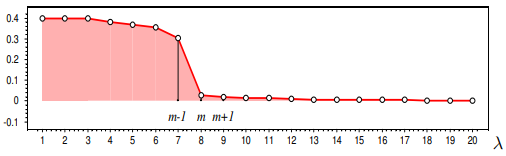
\includegraphics[width=1\linewidth]{Снимок экрана 2024-12-14 214833.png}
    \caption{Критерий крутого склона}
    \label{fig:enter-label}
\end{figure}

Математически можно записать, что эффективная размерность выборки - это наименьшее целое $m$, при котором: \par
$E_m = \frac{||GU^T-F||^2}{||F||^2} = \frac{\lambda_{m+1} + \dots + \lambda_{n}}{\lambda_{1} + \dots + \lambda_{n}} \leq \varepsilon$ \par

По этой картинке критерия крутого склона в моменте резкого падения можно найти $m$, после которого все значения будут близки к нулю. Это значит, что: $E_{m-1} \gg E_m$ и можно взять $m \leq n$ собственных значений и понизить размерность задачи. \par

А если крутого склона на графике нет? Если, например, у вас идёт монотонное, почти линейное снижение собственных значений до нуля это означает одно "--- никакой эффективной размерности у вас нет. Понизить размерность задачи линейными преобразованиями вам не удаётся и использовать МГК для такой задачи неприменим.

\section{Задачи на нахождение эффективной размерности выборки и их решение}
\begin{enumerate}
    \item \textbf{Задача про матрицу} \par
    Определить применим ли метод PCA для набора данных о 20 A  с 5ю характеристиками B, для которых матрица выглядит как:\par
     $\begin{pmatrix}
      4.4 &  0 & \cdots &  & 0 \\
      0  & 4.3 & 0 & \cdots &  0   \\
      0  & 0 & 4.2 & 0 & 0      \\
      0  & 0 & 0 & 4.1 & 0     \\
      0  & \cdots & \cdots & 0 & 4.0     \\
      0 & 0 & 0 & 0 & 0\\
      \vdots & \cdots & & \cdots &\vdots \\
      0 & 0 & 0 & 0 & 0\\
     \end{pmatrix}$ \par
     \textbf{Решение} \par
     \begin{itemize}
        \item найдём собственные значения и расположим их в убывающем порядке:\par
            \begin{itemize}
            \item $\lambda_{1}  = 4.0$
            \item $\lambda_{2}  = 4.1$
            \item $\lambda_{3}  = 4.2$
            \item $\lambda_{4}  = 4.3$
            \item $\lambda_{5}  = 4.4$
            \end{itemize}
        \item определим доли дисперсии по формуле $\frac{ \lambda_i }{\sum \lambda}$: \par
                \begin{itemize}
                \item $\frac{ \lambda_1 }{\sum \lambda}  = 0.1904$
                \item $\frac{ \lambda_2 }{\sum \lambda}  = 0.1952$
                \item $\frac{ \lambda_3 }{\sum \lambda}  = 0.2000$
                \item $\frac{ \lambda_4 }{\sum \lambda}  = 0.2048$
                \item $\frac{ \lambda_5 }{\sum \lambda}  = 0.2095$
            \end{itemize} \par
        \item построим график "крутого склона", где по оси OY откладывается значение долей дисперсии, а по оси OX "--- значение m. (Сам график опущен, мы уверены, что читатель справится построить его самостоятельно). \par
        \item по графику видно, что резкого падения или же крутого склона нет, а значит метод PCA для данных плохо применим.
     \end{itemize}\par
     \textbf{Ответ:} неприменим
    \item \textbf{Задача про анализы крови} \par
    Дан набор данных об анализах крови 15 пациентов с 5ю характеристиками (например, лейкоциты, эритроциты и тд), ковариационная матрица 15*5 представлена ниже. Определить применим ли метод PCA для этого набора данных и, если да, найти m "--- эффективную размерность выборки:\par    $\begin{pmatrix}
      2.1  & 1.8 & 1.2 & 0.9 & 0.7 \\
      1.9  & 1.6 & 1.1 & 0.8 & 0.6 \\
      1.8  & 1.5 & 1.0 & 0.7 & 0.5 \\
      1.7  & 1.4 & 0.9 & 0.6 & 0.4 \\
      1.6  & 1.3 & 0.8 & 0.5 & 0.3 \\
      1.5  & 1.2 & 0.7 & 0.4 & 0.2 \\
      1.4  & 1.1 & 0.6 & 0.3 & 0.1 \\
      1.3  & 1.0 & 0.5 & 0.2 & 0.1 \\
      1.2  & 0.9 & 0.4 & 0.1 & 0.1 \\
      1.1  & 0.8 & 0.3 & 0.1 & 0.1 \\
      1.0  & 0.7 & 0.2 & 0.1 & 0.1 \\
      0.9  & 0.6 & 0.2 & 0.1 & 0.1 \\
      0.8  & 0.5 & 0.2 & 0.1 & 0.1 \\
      0.7  & 0.4 & 0.2 & 0.1 & 0.1 \\
      0.6  & 0.3 & 0.2 & 0.1 & 0.1 \\
     \end{pmatrix}$ \par
     \textbf{Решение} \par
     \begin{itemize}
        \item найдём собственные значения и расположим их в убывающем порядке:\par
            \begin{itemize}
            \item $\lambda_{1}  = 5.2$
            \item $\lambda_{2}  = 3.1$
            \item $\lambda_{3}  = 0.8$
            \item $\lambda_{4}  = 0.5$
            \item $\lambda_{5}  = 0.4$
            \end{itemize}
        \item определим доли дисперсии по формуле $\frac{ \lambda_i }{\sum \lambda}$: \par
                \begin{itemize}
                \item $\frac{ \lambda_1 }{\sum \lambda}  = 0.52$
                \item $\frac{ \lambda_2 }{\sum \lambda}  = 0.31$
                \item $\frac{ \lambda_3 }{\sum \lambda}  = 0.08$
                \item $\frac{ \lambda_4 }{\sum \lambda}  = 0.05$
                \item $\frac{ \lambda_5 }{\sum \lambda}  = 0.04$
            \end{itemize} \par
        \item построим график "крутого склона", где по оси OY откладывается значение долей дисперсии, а по оси OX "--- значение m. (Сам график опущен, мы уверены, что читатель справится построить его самостоятельно). \par
        \item из графика видно, что есть резкий перегиб, то есть можно применить PCA
        \item Определим эффективные размерности, определяющие разные проценты выборки: \par
        \begin{itemize}
            \item 1 компонента даёт 52\%
            \item 2 компоненты дают 83\%
            \item 3 компоненты дают 91\%
            \item прибавление следующих компонент не внесёт серьёзный вклад
        \end{itemize}\par
        То есть для точности, например, в 80\% мы можем использовать размерность 2
    \end{itemize}
    \textbf{Ответ:} применим, для точности в 80\% достаточно размерности 2, а для точности 90\% "--- 3, дальнейшее повышение размерности (4 и полная размерность 5) не имеет смысла, так как усложняет вычисление задачи, но уточняет её несильно
    \item \textbf{Задача про машины} \par
    Дан набор данных о 1200 автомобилях с 14ю характеристиками (например: цвет, форма кузова, модель и др.), то есть матрица состоит из 1200 строк и 14 столбцов. Мы хотим использовать метод PCA для нахождения эффективной размерности выборки, чтобы, например, спрогнозировать цены на автомобили в зависимости от их характеристик. \par
    Шаги решения, которые мы предварительно применили:\par
    \begin{itemize}
        \item Отцентрировали данные, нашли средние значения характеристик
        \item Вычислили ковариационную матрицу
        \item Определили собственные значения и векторы. Собственные значения таковы: \par
        \begin{itemize}
            \item $\lambda_{1}  = 8.0$
            \item $\lambda_{2}  = 3.5$
            \item $\lambda_{3}  = 1.9$
            \item $\lambda_{4}  = 0.7$
            \item $\lambda_{5}  = 0.4$
            \item $\lambda_{6}  = 0.2$
            \item $\lambda_{7}  = 0.1$
            \item $\lambda_{8}  = 0.05$
            \item $\lambda_{9}  = 0.01$
            \item $\lambda_{10} = 0.005$
            \item $\lambda_{11} = 0.001$
            \item $\lambda_{12} = 0.0005$
            \item $\lambda_{13} = 0.0002$
            \item $\lambda_{14} = 0.0001$
        \end{itemize}
    \end{itemize}\par
    Доделайте задачу: \par
    \begin{itemize}
        \item Постройте график "крутого склона" и проведите анализ "сломанной трости"
        \item Найдите эффективную размерность, которая определяет 85\% общей дисперсии
    \end{itemize}\par
    \textbf{Решение} \par
    \begin{itemize}
        \item Предварительно нужно отсортировать по убывнию собственные значения $\lambda$. Проверили, на счастье, они уже расположены в нужном порядке. Теперь определим доли дисперсии по формуле $\frac{ \lambda_i }{\sum \lambda}$: \par
        \begin{itemize}
            \item $\frac{ \lambda_1 }{\sum \lambda}  = 0.538$
            \item $\frac{ \lambda_2 }{\sum \lambda}  = 0.235$
            \item $\frac{ \lambda_3 }{\sum \lambda}  = 0.127$
            \item $\frac{ \lambda_4 }{\sum \lambda}  = 0.047$
            \item $\frac{ \lambda_5 }{\sum \lambda}  = 0.027$
            \item $\frac{ \lambda_6 }{\sum \lambda} = 0.013$
            \item $\frac{ \lambda_7 }{\sum \lambda}  = 0.007$
            \item $\frac{ \lambda_8 }{\sum \lambda}  = 0.003$
            \item $\frac{ \lambda_9 }{\sum \lambda}  = 0.0006$
            \item $\frac{ \lambda_{10} }{\sum \lambda} = 0.0003$
            \item $\frac{ \lambda_{11} }{\sum \lambda} = 0.00006$
            \item $\frac{ \lambda_{12}}{\sum \lambda} = 0.00003$
            \item $\frac{ \lambda_{13} }{\sum \lambda} = 0.000013$
            \item $\frac{ \lambda_{14} }{\sum \lambda} = 0.000007$
        \end{itemize} \par
        По этим посчитанным данным строится график "крутого склона", где по оси OY откладывается значение долей дисперсии, а по оси OX "--- значение m. (Сам график опущен, мы уверены, что читатель справится построить его самостоятельно). \par
        Определяем точку перегиба, где всё стремится к нулю. Возле неё с заданной точностью будем определять эффективную размерность.
        \item Эффективная размерность, определяющая 85\% выборки соответсвует 3, так как: \par
        \begin{itemize}
            \item 1 компонента даёт 54\% (округлили 0,538 к доле 0,54 и записали в процентном соотношении)
            \item 2 компоненты дают 77\%
            \item 3 компоненты дают 90\%
        \end{itemize}\par
        \textbf{Ответ:} эффективная размерность "--- 3.
    \end{itemize}

\end{enumerate}

\section{Объясненная дисперсия после проекции. Проекция на пространство главных компонент, восстановление данных.}

\textbf{Метод главных компонент} (Principal Component Analysis, PCA) — это статистический метод преобразования пространства признаков, используемый для борьбы с мультаколлинеарностью в данных. В данном методе исходные признаки подвергаются некоторому функциональному преобразованию, при этом гарантируется линейная независимость новых признаков, и, возможное, сокращение их количества, то есть уменьшение размерности задачи. 

В методе главных компонент строится минимальное число новых признаков, по которым исходные признаки восстанавливаются линейным преобразованием с минимальными погрешностями. PCA относится к методам обучения без учителя (unsupervised learning), поскольку матрица «объекты–признаки» F преобразуется без учёта целевого вектора y.

Важно отметить, что PCA подходит и для регрессии, и для классификации, и для многих других типов задач анализа данных, как вспомогательное преобразование, позволяющее определить эффективную размерность исходных данных.

\textbf{Пусть}:

$f_1(x), ..., f_n(x)$ — исходные числовые признаки;

$g_1(x), ..., g_m(x)$ — новые числовые признаки, $m \leq n$;

\textbf{Требование}: старые признаки $f_i(x)$ должны линейно восстанавливаться по новым признакам $g_s(x)$:
\begin{equation}
    \hat{f}_j(x) = \sum_{i=1}^{m}g_s(x)u_{js}, \quad j = 1, ..., n, \quad \forall x \in X, 
\end{equation}
как можно точнее на обучающей выборке $x_1, ..., x_l$:
\begin{equation}
    \sum_{i=1}^{l}\sum_{j=1}^{n}(\hat{f}_j(x_i) - f_j(x_i))^{2} \rightarrow \underset{\{g_s(x_i)\}, \{u_{js}\}}{\min}
\end{equation}

Перейдем к матричным обозначениям. Матрицы объекты-признаки, старая и новая:
\begin{equation}
    \underset{l \times n}{F} = \begin{pmatrix} f_1(x_1) \quad ... \quad f_n(x_1) \\ ... \quad ... \quad ... \\ f_1(x_l) \quad ... \quad f_n(x_l) \end{pmatrix}; \quad \underset{l \times m}{G} = \begin{pmatrix} g_1(x_1) \quad ... \quad g_m(x_1) \\ ... \quad ... \quad ... \\ g_1(x_l) \quad ... \quad g_m(x_l) \end{pmatrix}.
\end{equation}
Матрица линейного преобразования новых признаков в старые:
\begin{equation}
    \underset{n \times m}{U} = \begin{pmatrix} u_{11} \quad ... \quad u_{1m} \\ ... \quad ... \quad ... \\ u_{n1} \quad ... \quad u_{nm} \end{pmatrix}; \quad \hat{F} = GU^{T} \approx F.
\end{equation}

\textbf{Цель}: найти и новые признаки G, и преобразование U по изветсной матрице F:
\begin{equation}
    \sum_{i=1}^{l}\sum_{j=1}^{n}(\hat{f}_j(x_i) - f_j(x_i))^{2} = \left\| GU^{T} - F \right\|^{2} \rightarrow \underset{G, U}{min},
\end{equation}

Решение помогает найти следующая теорема:

\textbf{Теорема}. Если $m \leq rk F$, то минимум $\left\| GU^{T} - F \right\|^{2}$ достигается, когда столбцы матрицы $U$ — это собственные векторы матрицы $F^{T}F$, соответствующие $m$ максимальным собственным значениям $\lambda_1, ..., \lambda_m$, а матрица $G = FU$.

При этом:

1. матрица $U$ ортонормирована: $U^{T}U = \hat{1}_m$;

2. матрица $G$ ортогональна: $G^{T}G = \Lambda = diag(\lambda_1, ..., \lambda_m)$;

3. $U \Lambda = F^{T}FU; G\Lambda = FF^{T}G$;

4. $\left\| GU^{T} - F \right\|^{2} = \left\|F\right\|^{2} - tr \Lambda = \sum_{j = m+1}^{n} \lambda_j$.

Таким образом, минимум функции $\left\| GU^{T} - F \right\|^{2}$ равен сумме наименьших собственных значений.

\textbf{Применение}: Сперва данные центрируются так, чтобы средние значения всех переменных были раны нулю, а именно:
\begin{equation}
    F_{centered} = F - \bar{F},
\end{equation}
где $F$ исходное признаковое описание данных, а $\bar{F}$ вектор средних значений по столбцам.

Далее происходит построение ковариационной матрицы:
\begin{equation}
    \Sigma = \frac{1}{n-1}F_{centered}^{T}F_{centered}.
\end{equation}

Следующий шаг — это найти собственные значения и собственные векторы ковариационной матрицы:
\begin{equation}
    \Sigma \mathbf{u_i} = \lambda_i \mathbf{u_i}.
\end{equation}
Впоследствии из них выбираются несколько главных компонент (собственных векторов), соответствующих наибольшим собственным значениям, объясняющих большую часть данных.

Последним шагом является проецирование исходных данных на главные компоненты:
\begin{equation}
    Z = F_{centered}U_k,
\end{equation}
где $U_k$ — матрица $k$ отобранных собственных вектров (главных компонент), Z — это матрица исходных данных, представленных в пространстве главных компонент.

\textbf{Объясненная дисперсия}. Для оценки меры того, насколько признаки в новом пространстве хорошо описывают исходные данные используется объясненная дисперсия. Объясненная дисперсия отражает долю общей дисперсии зависимой переменной, которая может быть объяснена независимыми переменными в модели. 
\begin{equation}
    \text{Объясненная дисперсия} = \frac{\sum_{i=1}^{k}\lambda_i}{\sum_{i=1}^{n}\lambda_i}.
\end{equation}

\textbf{Восстановление исходных данных}. Для восстановления исходных данных используется следующая формула:
\begin{equation}
    F_{reconstructed} = Z U_{k}^{T} + \bar{F}, 
\end{equation}
где Z — матрица проекций на главные компоненты.

При восстановлении данных всегда возникает ошибка, которая определяется как разница между исходными данными и восстановленными данными. Эта ошибка может быть измерена с помощью среднеквадратичной ошибки (MSE):
\begin{equation}
    MSE = \frac{1}{n} \sum_{i = 1}{l} \left\|F_i - F_{reconstructed, i} \right\|^{2},
\end{equation}
где l — количество наблюдений, $F_i$ — исходные данные, а $F_{reconstructed}$ — восстановленные данные.

\textbf{Задача 1.}

\textit{Условие}. Рассмотрим набор данных с тремя признаками $X_1, X_2, X_3$ с матрицей ковариации:
\begin{equation}
    \Sigma = \begin{pmatrix} 4 \quad 2 \quad 0 \\ 4 \quad 3 \quad 1 \\ 0 \quad 1 \quad 2 \end{pmatrix}.
\end{equation}
Найдите долю объясненной дисперсии, приходящейся на каждую лавную главную компоненту.

\textit{Решение}. Найдем собственные значения матрицы ковариации:
\begin{equation}
    det \begin{pmatrix} 4 - \lambda \quad 2 \quad 0 \\ 4 \quad 3 - \lambda \quad 1 \\ 0 \quad 1 \quad 2 - \lambda \end{pmatrix} = 0 \quad \rightarrow \quad \lambda_1 = 0, \lambda_2 = 2, \lambda_3 = 6.
\end{equation}
Найдем долю объясненной дисперсии, приходящейся на каждую лавную главную компоненту:
\begin{equation}
    \text{Доля}_1 = \frac{\lambda_1}{\lambda_1 + \lambda_2 + \lambda_3} = \frac{0}{0 + 2 + 6} = 0,
\end{equation}
\begin{equation}
    \text{Доля}_2 = \frac{\lambda_2}{\lambda_1 + \lambda_2 + \lambda_3} = \frac{2}{0 + 2 + 6} = 0.25,
\end{equation}
\begin{equation}
    \text{Доля}_3 = \frac{\lambda_3}{\lambda_1 + \lambda_2 + \lambda_3} = \frac{6}{0 + 2 + 6} = 0.75.
\end{equation}

\textbf{Задача 2.}

\textit{Условие}. Рассмотрим набор данных с двумя признаками $(X1, X2)$: $X_1 = (-1, -1, 2), X_2 = (2, -1, -1)$. Найдите проекцию данных на первую главную компоненту.

\textit{Решение}. 1. Центрирование данных. Средние значения: 
\begin{equation}
    \bar{X}_1 = \frac{-1 - 1 + 2}{3} = 0 \quad \bar{X}_2 = \frac{2 - 1 - 1}{3} = 0.
\end{equation}
Центрированные данные: 
\begin{equation}
    X_{centered} = \begin{pmatrix} -1 & 2 \\ -1 &  -1 \\ 2 & -1 \end{pmatrix}.
\end{equation}

2. Вычисление ковариационной матрицы. Ковариационная матрица $C$ вычисляется как:
\begin{equation}
    \Sigma = \frac{1}{n-1}X_{centered}^{T}X_{centered},
\end{equation}
где $n = 5$ - количество наблюдений.
После расчетов получаем:
\begin{equation}
    \Sigma = \begin{pmatrix} \text{Var}(X_1) & \text{Cov}(X_1, X_2) \\ \text{Cov}(X_1, X_2) & \text{Var}(X_2) \end{pmatrix} = \begin{pmatrix} 1.5 & -0.75 \\ -0.75 & 1.5 \end{pmatrix}
\end{equation}

3. Решая характеристическое уравнение $|\Sigma - \lambda \hat{1}| = 0$ находим собственные значения: $\lambda_1 = 0.75, \quad \lambda_2 = 2.25$.

Собственные векторы соответствующие этим собственным: $u_1 = (1, 1), \quad u_2 = (-1, 1)$.

4. Проекция на первую главную компоненту. Проекция данных на первую главную компоненту осуществляется следующим образом: $Z = X_{centered} v_1^T$. После вычислений получаем проекцию: $Z =\begin{pmatrix} 1 \\ -2 \\ 1 \end{pmatrix}$.

\textbf{Задача 3.}

\textit{Условие}. В задаче 2 восстановите исходные данные из полученной проекции.

\textit{Решение}. Для восстановления данных используем формулу: 
\begin{equation}
    X_{reconstructed} = Zu_1 + \bar{X},
\end{equation}
 где $\bar{X} = (0, 0)$.

 Тогда $X_{1, reconstructed} = (1, -2, 1), X_{1, reconstructed} = (-1, 2, -1)$.


\section{Анализ соответствий}
\textbf{Анализ соответствий (Correspondence analysis (CA)} — обобщение метода главных компонент, предназначенное для работы с
категориальными признаками. Другие имена, существующие из-за того, что технику CA часто переоткрвали -- "dual scaling,” “optimal scaling,” “homogeneity analysis” или “reciprocal averaging". CA отображает матрицу признаков в два множество новых переменных, которые называются "factor scores".\\
Factor scores  дают подобраны так, что они оптимальным образом отображают похожесть строк (первое множество) и столбцов (второе) изначальной таблицы. В двух множествах роль factor scores играют точки, чьи  измерения также называют \textit{компонентами}, что подчёркивает связь с PCA. Если быть точнее, factor scores отвечают за вклад каждой из ортогональных компонент в итоговую матрицу.\\
В силу нехватки места, будем детально рассматривать CA для 2х категориальных признаков.\\
Мы будем анализировать данные сразу по таблице сопряжённости, т.е. таблици типа 
\begin{table}[H]\centering
\begin{tabular}{|c|c|c|}
\hline  & Right-handed & Left-handed  \\
\hline Male & 43 & 9 \\
\hline Female & 44 & 4  \\
\hline
\end{tabular}
\end{table}
\subsection{Описание метода}
Для начала преобразуем таблицу в матрицу вероятностей. Для этого разделим все элементы матрицы на сумму матрицы и получим матрицу \textbf{Z}.\\
Пусть $r=Z\textbf{1}$, $c=Z^T\textbf{1}$. Затем пусть $D_c=\text{diag\{c\}}$, $D_r=\text{diag\{r\}}$.\\
Теперь рассмотрим матрицу $S=D_r^{-1/2}(Z-rc^T)D_c^{-1/2}$.
Разложим матрицу по SVD (сингулярное разложение)
$$S=P\Delta Q^T$$
Матрица P (соответственно Q) содержит левые
(соответственно правые) сингулярные векторы матрицы $S$. Диагональные элементы
диагональной матрицы $\Delta$ являются её сингулярными значениями. 
По свойствам SVD, аналогично PCA, квадраты сингулярных значений будут собственными значениями матрицы $S^TS$; пусть $\Lambda=\Delta^2$. Эти собственные значения, все так же, как в PCA, выражают дисперсию, соответствующим фактором, а их сумма называется общей инерцией изначальной матрицы.\\
Теперь factor scores получаются по следующей формуле:
$$F=D_r^{-1/2}P\Delta\text{ и }G=D_c^{-1/2}Q\Delta$$
(раньше, в PCA, была одна марица из $X=P\Delta Q^T$, равная $F'=P\Delta$, для неё $F'=P\Delta=XQ$; $X=F'Q^T$, т.е. ортогональная матрица $Q^T$ по сути то, куда мы проецируем).
\subsection{Что тут оптимального?}
Критерий, по которому CA оптимален -- дисперсия factor scores. Например, первая строка $f_1$ у матрицы $F$ -- линейная комбинация столбцов $Z-rc^T$, с ограничениями от $D_r^{-1/2}$, $D_c^{-1/2}$, точнее $$f_1=D^{-1}_r(Z-rc^T)D^{-1}_cq_1$$$$\textbf{s.t.} f_1=\arg\max\limits_{f}f^TD_rf$$$$ q_1^TD_c^{-1}q_1=1$$  
Не менее важное свойства CA -- то, что он оптимален \textit{с точки зрения $\chi^2$}. Точнее, общая инерция строк пропорционально $\chi^2$ из теста Пирсона для нуль-гипотезы того, что строки и столбцы независимы:
$$\chi^2=N\sum_i^I\sum_j^J\frac{(z_{ij}-r_ic_j)^2}{r_ic_j}=N\phi^2$$.\\
Как следует из курса статистики, при верности нуль-гипотезы этот притерий имеет распределение $\chi^2\left((I-1)(J-1)\right)$, и с его помощью можно проверять нуль-гипотезу.\\
Общая инерция матрицы $S$ вычисляется по следующей формуле:
$$\mathcal{I}=\text{tr}\left\{S^TS\right\}=\sum_i^I\sum_j^J\frac{(z_{ij}-r_ic_j)^2}{r_ic_j}=\phi^2$$
Таким образом, факторы СА выполняют ортогональное разложение критерия $\chi^2$, где каждый фактор "объясняет" часть отклонение от независимости строк.
Ещё одно свойство, то, что дисперсия factor scores для всех строк и столбцов одинакова. И вообще, можно получить F из G и G из F:
$$F=D_r^{-1/2}P\Delta=D_r^{-1/2}SQ=D_r^{-1}(Z-rc^T)D_c^{-1/2}Q=D_r^{-1}(Z-rc^T)G\Delta^{-1}=D_r^{-1}ZG\Delta^{-1}-D_r^{-1}rc^TG\Delta^{-1}$$
А затем, по построениею $r$ и $c$, вторая компонента равна 0, а значит
$$F=D_r^{-1}ZG\Delta^{-1}$$
Аналогично $$G=D_c^{-1}Z^TF\Delta^{-1}$$.
\section{Некоторые задачи на анализ соответствий}
\subsection{Задачи по анализу соответствий}
\problem Пусть $X\in\mathbb{R}_{nxp}$ -- таблица сопряженности. Понять, какую значимость имеет каждый признак. Даны следующие данные.
(Подсказка: нужно поситать пропорцию инерций, как в 1 задаче для PCA)

a) \begin{table}[H]\centering
\begin{tabular}{ccc}
\toprule
Right-handed & Left-handed  \\
\midrule Male & 43 & 9 \\
Female & 44 & 4  \\
\bottomrule
\end{tabular}
\caption{Распределение левшей и правшей}
\end{table}

b) Матрица побольше \begin{table}[H]
\centering
\begin{tabular}{cccc}
\toprule
Level of education  &  Glance & Fairly thorough & Very thorough\\
\midrule  
  Some primary      &    5    &    7  & 2\\
  Primary completed   &  18    &    46 & 20\\
  Some secondary  &  19        & 29  & 39\\
  Secondary completed & 12    &  40  &   49\\
  Some tertiary &  3 &    7 &  16\\
\bottomrule
\end{tabular}
\caption{Умения читать}
\end{table}
\problem Показать, что у матрицы $\Delta$ диагональные элементы все меньше 1.
Подсказка: воспользоваться связью между $F$ и $G$
Примечание: почти вся теория взята из статьи Correspondence Analysis (Adbi, Bera)
